
\section{Kennismaken met de Arduino omgeving}

De Arduino omgeving oftewel Arduino IDE (Integrated Development Environment) kan je gebruiken om de Microbit te programmeren. 
%Mocht je de software nog niet geïnstalleerd hebben, volg dan de instructies in “Installatiehandleiding Arduino software voor BBC Microbit”.

We gebruiken de Arduino IDE omdat deze op beginnersniveau zeer veel gebruikt wordt en er veel voorbeeldcode te vinden is.
 
Eigenlijk maakt de Arduino IDE gebruik van de taal C++, dit is een Object Oriented uitbreiding van de taal C. Het C++ / Object Oriented deel van de programmeertaal zie je soms terug in instructies zoals Serial.begin(9600); De punt tussen Serial en begin is hier een indicatie van.

Java en C++ zijn object georiënteerde talen. Daarover leer je meer als je kiest voor de differentiaties “Software Engineering” of “Networks \& System Engineering”. Voor dit practicum houden we het eenvoudig. We gebruiken de taal zoveel mogelijk als klassieke “imperatieve” programmeertaal waarbij gewerkt wordt met een reeks opeenvolgende instructies.

%Voorheen maakten we gebruik van een Arduino Uno. We zijn overgestapt naar de Microbit omdat deze veel meer mogelijkheden biedt zoals meer ingebouwde sensoren en Bluetooth en ook nog eens goedkoper is dan een Arduino. 
%De Microbit is een IoT device (Internet of Things). Daardoor kun je in ‘The Challenge’ veel meer met een Microbit dan met een Arduino Uno.



\subsection{Het installeren van de Arduino omgeving}

VOER ONDERSTAANDE INSTALLATIE THUIS UIT – DIT DUURT 1,5 UUR!!!

\begin{enumerate}
	\item Download de Arduino software van \href{https://https://www.arduino.cc/en/software}{https://www.arduino.cc/en/software}, zoals je kan zien zijn er ook versies voor Linux en de Mac.
	\item Kies de Windows installer, niet de app. De app is niet geschikt voor wat wij gaan doen.
	\item  Bevestig alle vragen, klik maar door.
\end{enumerate}

Instellingen wijzigen: Ga naar File $\rightarrow$ Preferences $\rightarrow$ Sketchbook location, zoals te zien in figuur \ref{fig:arduinoPref}, en wijzig het pad:
\begin{figure}[h!]
	\captionsetup{justification=centering}
	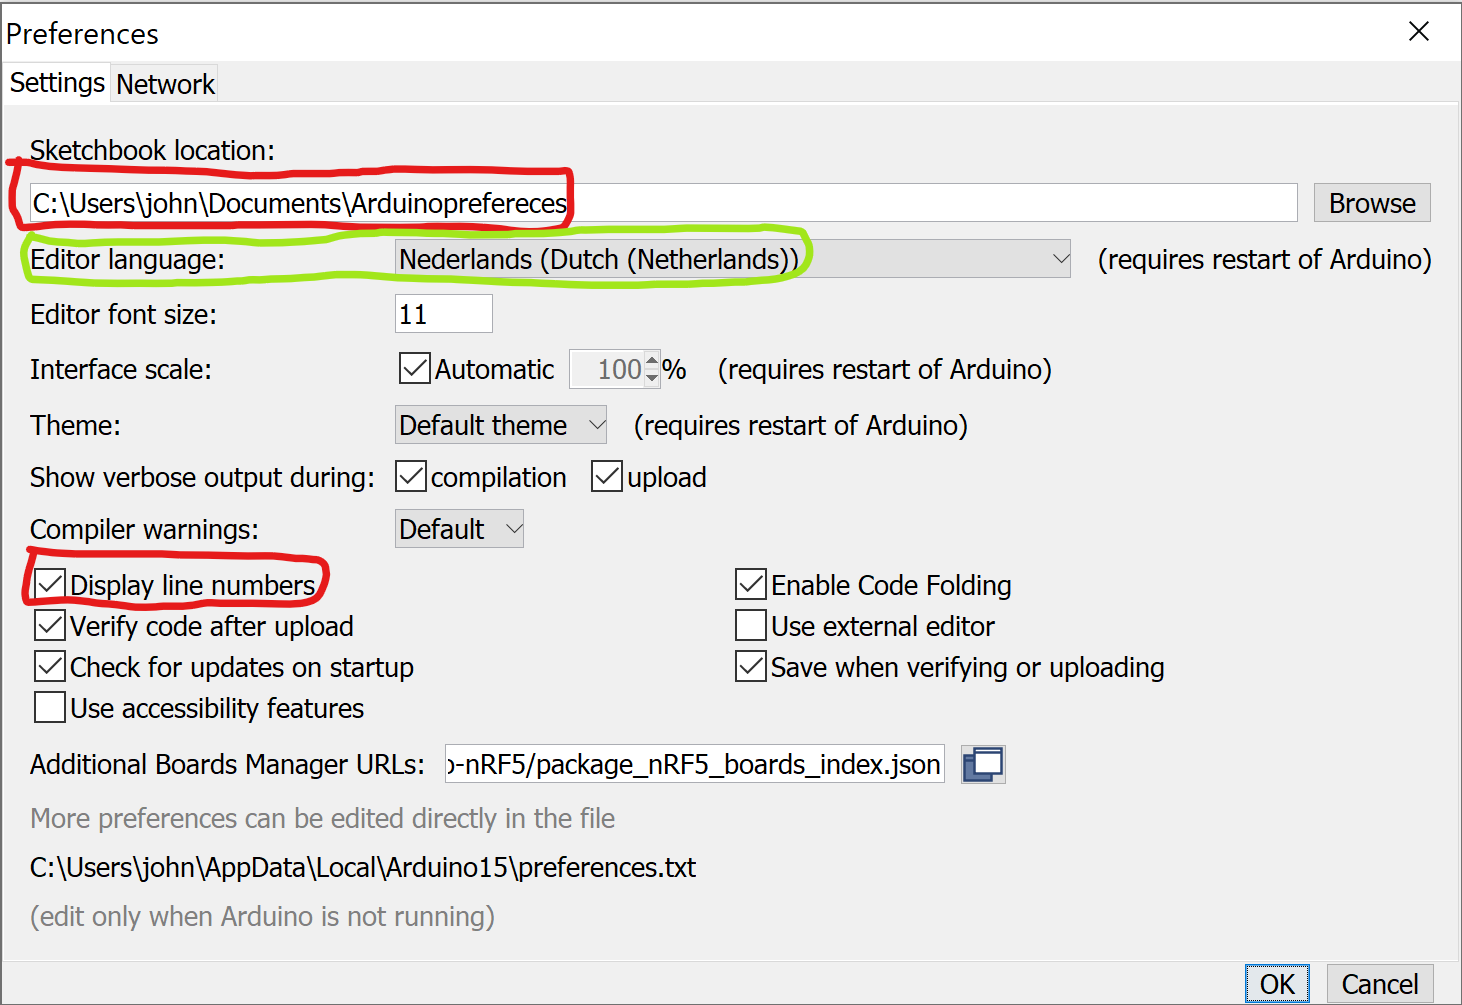
\includegraphics[width=0.50 \linewidth]{figuren/arduinoPref}
	\centering
	\caption{preferences scherm.}
	\label{fig:arduinoPref}
\end{figure}

\begin{itemize}
	\item C:\textbackslash Users\textbackslash \textit{john}\textbackslash Documents\textbackslash Arduino (in mijn geval)
	\item Zet “Display line numbers” aan.
	\item Indien de Arduino omgeving Engelstalig is, kan deze gewijzigd worden naar het Nederlands. Het is handig om tijdens de installatie de Engelstalige omgeving te gebruiken.
\end{itemize}


\subsection{De arduino omgeving geschikt maken voor de microbit.}

De firma \href{https://www.adafruit.com/about}{Adafruit } ontwikkelt diverse componenten voor met name embedded systemen
die door ieder gebruiker kan worden toegepast en/of geprogrammeerd. Om dit waar te kunnen maken worden veel tutorials ontwikkeld. Zo is er ook een uitgebreide website, om de \href{https://learn.adafruit.com/use-micro-bit-with-arduino}{microbit met de Arduino IDE} te programmeren.
\begin{enumerate}
	\item Ga naar de Adafruit website om  de \href{https://learn.adafruit.com/use-micro-bit-with-arduino}{microbit met de Arduino IDE} te programmeren.
	\item Scroll naar beneden en klik op \fcolorbox{black}{NavyBlue}{\textcolor{White}{\textbf{Install board and blink! \textgreater}}}. Voer vervolgens het onderdeel "Add NRF5x Board Support" uit (dit kan een enige tijd duren, raak niet in paniek en neem wat te drinken). Nadat de installatie gebeurd is wordt dit door Adafruit uitgetest met het programmaatje blink. Het werken met het programma blink wordt gedaan bij punt \ref{en:blink}.
	
	\item Het selecteren van de BBC micro:bit V2 board en de USB port.
	\begin{enumerate}
		\item Selecteer BBC micro:bit V2.
		\begin{figure}[h!]
			\captionsetup{justification=centering}
			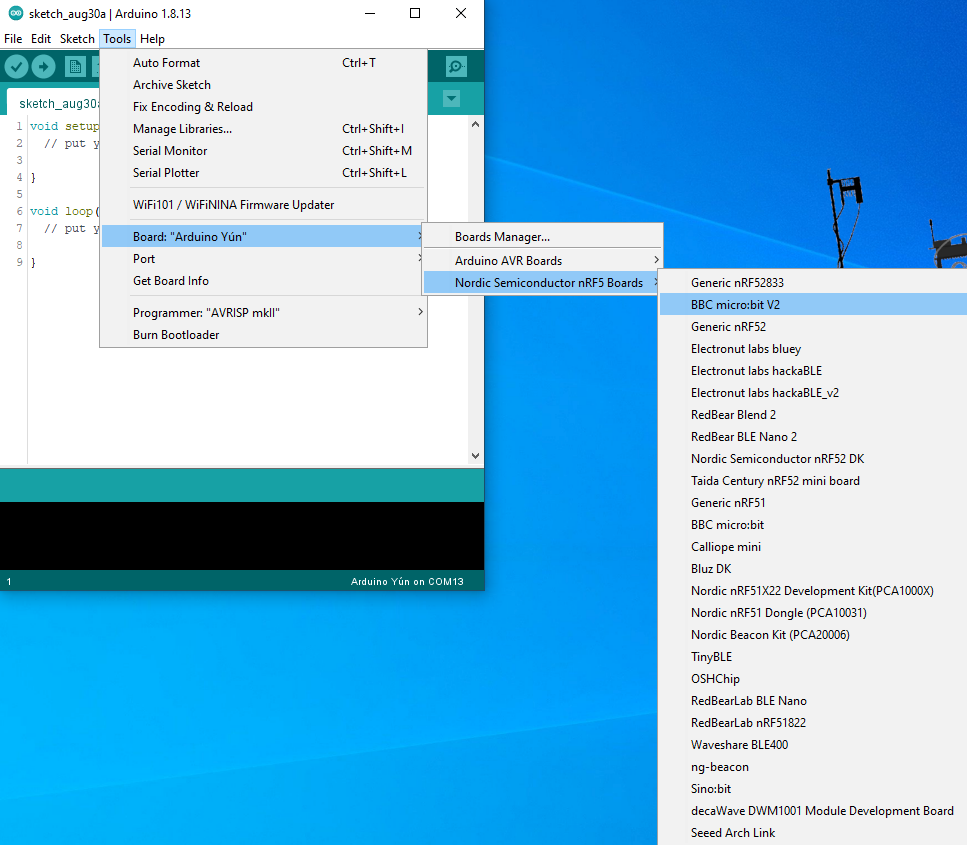
\includegraphics[width=0.45 \linewidth]{figuren/selBBCV2}
			\centering
			\caption{Selecteren van de BBC micro:bit V2.}
			\label{fig:selBoard}
		\end{figure}
	    \item Het setten van de USB port.
	     	\begin{figure}[h!]
	     	\captionsetup{justification=centering}
	     	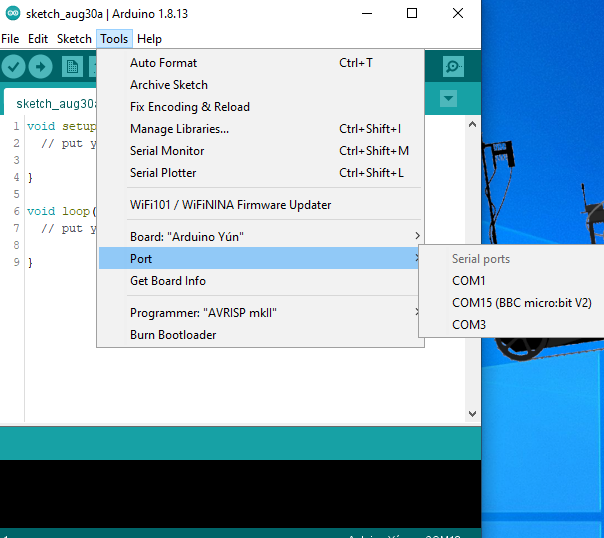
\includegraphics[width=0.45 \linewidth]{figuren/selBBCPort}
	     	\centering
	     	\caption{Selecteren van de USB port.}
	     	\label{fig:selUSB}
	     \end{figure}
     Indien de microbit niet herkent wordt, start de arduino omgeving opnieuw op en/of plug de microbit opnieuw in de USB poort.
	\end{enumerate}
~ 
   \item Het uploaden van een programma gebeurt door op de knop \img{figuren/ardIcUpl} te klikken. Windows komt met de melding zoals hieronder wordt weergegeven. 
   	\begin{figure}[h!]
   	\captionsetup{justification=centering}
   	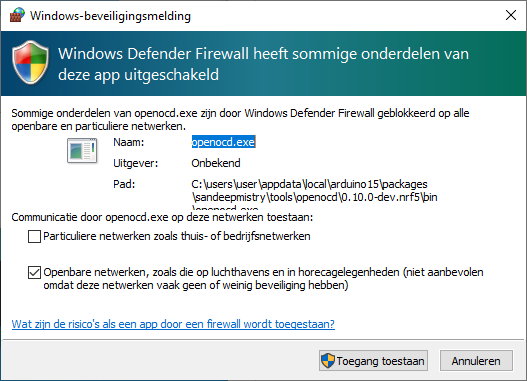
\includegraphics[width=0.45 \linewidth]{figuren/windowsDefSec}
   	\centering
   	\caption{Melding van windows defender.}
   	\label{fig:windowsDef}
   \end{figure}
Hiermee vraagt Windows toestemming om de USB port te mogen gebruiken.
\item Haal de voorbeeldcode van blackboard of \href{http://home.caiway.nl/~johnvi/embeddedFirstSem/voorbeeldCodeEmbedded.zip}{download} de laatste versie en plaats deze in je eigen werkdirectory.
\item \label{en:blink} Open het voorbeeldprogramma blink.ino (dubbel klik), dat wordt weergegeven in Listing \ref{lst:blink}, compileer en upload naar de micro:bit (klik op de knop \img{figuren/ardIcUpl}). \\
Als het goed is gaat het linkerboven LEDje van de matrix knipperen.

\end{enumerate}



